% Template for APA submission with R Markdown

% Stuff changed from PLOS Template
\documentclass[a4paper,man,apacite,floatsintext]{apa6}
\usepackage{apacite}

% amsmath package, useful for mathematical formulas
\usepackage{amsmath}
% amssymb package, useful for mathematical symbols
\usepackage{amssymb}

% hyperref package, useful for hyperlinks
\usepackage{hyperref}

% graphicx package, useful for including eps and pdf graphics
% include graphics with the command \includegraphics
\usepackage{graphicx}

% Sweave(-like)
\usepackage{fancyvrb}
\DefineVerbatimEnvironment{Sinput}{Verbatim}{fontshape=sl}
\DefineVerbatimEnvironment{Soutput}{Verbatim}{}
\DefineVerbatimEnvironment{Scode}{Verbatim}{fontshape=sl}
\newenvironment{Schunk}{}{}
\DefineVerbatimEnvironment{Code}{Verbatim}{}
\DefineVerbatimEnvironment{CodeInput}{Verbatim}{fontshape=sl}
\DefineVerbatimEnvironment{CodeOutput}{Verbatim}{}
\newenvironment{CodeChunk}{}{}

% cite package, to clean up citations in the main text. Do not remove.
\usepackage{cite}

\usepackage{color}

% Use doublespacing - comment out for single spacing
%\usepackage{setspace}
%\doublespacing


% Text layout
\topmargin 0.0cm
\oddsidemargin 0.5cm
\evensidemargin 0.5cm
\textwidth 16cm
\textheight 21cm

% Bold the 'Figure #' in the caption and separate it with a period
% Captions will be left justified
\usepackage[labelfont=bf,labelsep=period,justification=raggedright]{caption}


% Remove brackets from numbering in List of References
\makeatletter
\renewcommand{\@biblabel}[1]{\quad#1.}
\makeatother


% Leave date blank
\date{}

%\pagestyle{myheadings}
%% ** EDIT HERE **


%% ** EDIT HERE **
%% PLEASE INCLUDE ALL MACROS BELOW

%% END MACROS SECTION


% ALL OF THE TITLE PAGE INFORMATION IS SPECIFIED IN THE YAML
\title{\textbf{Developmental Gains in Speed and Accuracy in the Processing of Ad-Hoc
Implicatures}}
\shorttitle{Children's ad-hoc implicature processing}

\author{Erica J. Yoon, Michael C. Frank}

\affiliation{Department of Psychology, Stanford University}

\authornote{We would like to acknowledge Asher Kaye and Stephanie Hsiang for their
assistance in data collection, and thank the staff and families at
Children's Discovery Museum of San Jose and Bing Nursery School. Address
all correspondence to Erica J. Yoon, Stanford University, Department of
Psychology, Jordan Hall, 450 Serra Mall (Bldg. 420), Stanford, CA,
94305. E-mail:
\href{mailto:ejyoon@stanford.edu}{\nolinkurl{ejyoon@stanford.edu}}.}
\abstract{Language comprehension often requires making \emph{implicatures}: for
example, inferring that ``I ate some of the cookies'' implies the
speaker ate some \emph{but not all} (scalar implicatures); and ``I ate
the chocolate-chip cookies'' where there are both chocolate chip cookies
and raisin cookies in the context implies that the speaker ate the
chocolate chip, \emph{but not both the chocolate chip and raisin
cookies} (ad-hoc implicatures). Developmental work have reported mixed
results about the development of implicature processing abilities. In
the current work we use time-sensitive methods (eye-tracking and tablet)
to examine developmental gains in children's ad-hoc implicature
processing, and test whether one cause of toddlers' consistent failure
to process implicature is their difficulty with executive function -
specifically inhibitory control to inhibit responses toward a salient
distractor (\emph{inhibitory hypothesis}). Across three experiments, we
present evidence for successful implicature computation by children as
young as 3 years, substantial developmental gains in implicature
computation from 2 to 5 years in both paradigms, and support for the
inhibitory hypothesis. Our work contributes to the growing literature of
early signs of pragmatic understanding in children.}
\keywords{Pragmatics; cognitive development; language processing; implicature;
inhibitory control; eye-tracking; tablet}

\begin{document}
\maketitle

\section{Introduction}\label{introduction}

Language comprehension often requires inferring speakers' intended
meanings that go beyond the literal meanings of what they say. In Grice
(1975)'s account, conversation is a cooperative act: A speaker will
cooperatively choose utterances such that the listener can understand
the intended message, and the listener will interpret the utterance with
this assumption of the speaker's cooperativeness in mind. According to
Grice (1975), a key maxim observed in cooperative communication is that
the speaker makes the contribution as informative as is required by the
conversation at hand. Thus, expecting a cooperative speaker to have
produced a maximally informative utterance, the listener can make
inferences that go beyond the literal meanings of the speaker's words.

The non-literal meanings computed through these inferential processes
are called pragmatic implicatures. For example, ``I ate some of the
cookies'' implies that the speaker ate some but not all of the cookies,
because a cooperative speaker who ate all would have said ``all,'' which
is more informative than the weaker alternative ``some.'' This is an
example of a scalar implicature, in which use of a weaker term
(``some'') in a lexical scale negates a stronger alternative (``all'').
Another kind of implicature is context-based, ad-hoc implicatures: ``I
ate the chocolate chip cookies'' in a context where two kinds of cookies
are available, chocolate chip and raisin, implies that the speaker ate
the chocolate-chip but not both the chocolate chip cookies and raisin
cookies. In this case, the context sets up a contrast between the term
offered (``chocolate chip cookie'') and the stronger alternative to be
negated (``chocolate chip and raisin cookies'')\footnote{Grice (1975)
  calls these implicatures \emph{generalized} (scalar) vs.
  \emph{particularized} (ad-hoc), but we use a theory-neutral
  designation here.}.

Simple implicatures like these have been an important case study for
pragmatics more broadly. Both classic, informal models of communication
(e.g., Grice, 1975; Sperber \& Wilson, 1995) and more recent
probabilistic models of pragmatic inference (e.g., Frank \& Goodman,
2012; Goodman \& Stuhlmuller, 2013) describe the processes that language
users use to compute such implicatures. And a rich psycholinguistic
literature has measured adults' processing of implicatures relative to
literal interpretations and found that adults robustly compute
implicatures, albeit more slowly than unambiguous literal meanings
(Bott, Bailey, \& Grodner, 2012; Breheny, Ferguson, \& Katsos, 2013;
Huang \& Snedeker, 2009a).

How does the ability to make implicatures develop? Since implicature
computation is an important indicator of broader pragmatic
understanding, many studies have extensively tested children's
abilities. To date, findings have been mixed, with children especially
struggling with scalar implicatures. For example, in Papafragou \&
Musolino (2003)'s study, a puppet saw three out of three horses jumped
over a fence, and described the scene by saying ``Some of the horses
jumped over the fence.'' When asked whether the statement is a good
description of the context at hand, adults rejected the infelicitous
statement whereas children mostly accepted it, which suggested that
children failed to compute \emph{some} vs. \emph{all} implicatures
(though see Katsos \& Bishop (2011), for an alternative explanation).
Besides struggling with \emph{some} vs. \emph{all} (Huang \& Snedeker,
2009b; Hurewitz, Papafragou, Gleitman, \& Gelman, 2006; Noveck, 2001),
children have consistently failed to compute implicatures involving
scalar contrasts, including \emph{a} vs. \emph{some} (Barner, Chow, \&
Yang, 2009), \emph{might} vs. \emph{must} (Noveck, 2001), and \emph{or}
vs. \emph{and} (Chierchia, Crain, Guasti, Gualmini, \& Meroni, 2001).

While children struggle on many scalar implicature tasks, they tend to
be more successful at computing ad-hoc implicatures (which depend on
context, rather than lexical scales). One potential difficulty in a
typical scalar implicature task is the need to generate relevant
alternatives to a given scalar term. For children to hear ``some of the
horses jumped over the fence'' and derive the implicature ``some
\emph{but not all},'' they must first realize that ``all'' is the
relevant alternative to ``some''. Barner, Brooks, \& Bale (2011) argued
that children's failures in the scalar implicature tasks are due to
their lack of ability to spontaneously generate the alternative to
negate upon hearing the term offered. Barner et al. (2011)'s claim
predicts that children's implicature computation should improve when
they can access the relevant alternatives. Consistent with this
hypothesis, children show substantially improved implicature computation
in ad-hoc implicature tasks -- which provided access to relevant
alternatives in context -- compared to scalar implicature tasks
(Horowitz, Schneider, \& Frank, under review; Katsos \& Bishop, 2011;
Papafragou \& Tantalou, 2004; Stiller, Goodman, \& Frank, 2015).

For example, Stiller et al. (2015) showed 2.5- to 5-year-old children
three different faces: a face with no item; a face with only glasses;
and a face with glasses and top-hat, and asked children to choose one of
the three faces as the referent in a puppet's statement, ``My friend has
glasses.'' Thus there was no need for children to spontaneously generate
the alternative (``glasses and top-hat'') to the term used (``glasses'')
because the alternative was visible in the context. In this task,
children as young as 3.5 years chose the face with only glasses as the
referent, which shows they successfully computed the implicature that
the puppet's friend has ``glasses \emph{but not both glasses and
top-hat}.'' Similarly, in Horowitz et al. (under review)'s study that
tested both children's scalar and ad-hoc implicature computation,
4-year-olds successfully made ad-hoc implicatures, but performed poorly
on scalar implicatures.

Despite older children's success, toddlers below 3 years struggle with
ad-hoc implicatures. Even Stiller et al. (2015)'s paradigm, which found
evidence of implicatures in the youngest ages to date, 2.5- and
3-year-olds still failed to compute implicatures. But does this finding
imply that the young toddlers lack pragmatic understanding, specifically
an awareness of the need for informativeness in cooperative
communication? On the contrary, children are sensitive to
informativeness in communication: From age two onward, when they are
asked to produce referring expressions, children recognize the level of
referential ambiguity and attempt to provide more information through
speech and gestures when the ambiguity level is greater (Matthews,
Butcher, Lieven, \& Tomasello, 2012; O'Neill \& Topolovec, 2001). Hence,
lack of sensitivity to the need for communicative informativeness does
not seem to be the problem for toddlers' implicature processing. So what
causes toddlers' failures in ad-hoc implicature tasks?

One potential candidate is children's lack of inhibitory control, or
inability to inhibit their selection of salient objects in the context.
Scalar implicature is typically described as requires rejecting a
stronger meaning (e.g., ``all'') and adding its negation to the weaker
term (e.g., ``some but not all''). In a task based on referent
selection, participants need to suppress selecting a distractor that
represents the stronger meaning, and thus has a larger set size (all of
the cookies) or more features (hat and glasses) and is more salient.
Instead they must choose a less salient target that represents the
weaker meaning (some of the cookies, glasses only). This kind of task
may be challenging to children because their executive function --
specifically their ability to inhibit responses to salient targets -- is
not yet fully developed (Davidson, Amso, Anderson, \& Diamond, 2006;
Diamond \& Taylor, 1996).

Processing measures may help to identify potential sources of difficulty
in pragmatic tasks, including issues in inhibitory control. Many
previous implicature tasks have measured only the accuracy of children's
responses. For example, studies often use as their sole dependent
measure whether children correctly judge a statement to be felicitous or
infelicitous, or whether they accurately select a felicitous referent
(\emph{target}) vs.~an incorrect counterpart (\emph{distractor}). Since
implicature has been argued to be a time-consuming computation (at least
in some contexts; Bott et al., 2012; Huang \& Snedeker, 2009a), adding a
time dimension to these accuracy measures might help provide a fuller
account of children's inferential process. In particular, examining
children's allocation of attention to targets and distractor at
different phases of utterance processing might help identify specific
aspects of the task as contributing to children's decision-making
process (e.g., the salience of a particular target).

Eye-tracking and tablet paradigms allow analyses of accuracy and
reaction time measures. Eye-tracking allows moment-by-moment analysis of
the trajectory of eye gaze, which may provide insight into children's
reasoning at intermediate stages of the inferential process. For
example, one set of implicature tasks used eye-tracking to show that
both adults and children were delayed in identifying the inferential
(compared to unambiguous) target; however, adults, but not children,
computed scalar implicatures rapidly enough to identify the inferential
target before the referent is semantically (literally) disambiguated in
the utterance (Huang \& Snedeker, 2009a, 2009b). Thus, eye-tracking
makes it possible to compare group performances at a precise time
interval given. While they do not yield moment-to-moment trajectories,
tablet paradigms have some of the advantages of both naturalistic and
time-sensitive paradigms. They resemble studies with storybook stimuli
that are familiar to children, and interaction with the touchscreen
keeps the task engaging. Tablets also make it possible to record the
amount of time before the subject made a decision, allowing
time-sensitive analyses of children's pragmatic processing (Frank,
Sugarman, Horowitz, Lewis, \& Yurovsky, 2016).

Consistent with the idea that some type of inhibitory control issue
might play a role in children's implicature computation, other
eye-tracking studies of language processing have shown that young
children have difficulty in allocating attention toward targets that are
less perceptually salient (e.g., Hollich et al., 2000; Nordmeyer \&
Frank, 2014; Pruden, Hirsh-Pasek, Golinkoff, \& Hennon, 2006; Yurovsky
\& Frank, 2015). For example, in Yurovsky \& Frank (2015), 1.5- to
2-year-olds showed evidence of word learning when the target (the
correct referent of the newly-learned word) and distractor (previously
unnamed named object) were matched in perceptual salience, but when
salience was greater for the distractor, word learning abilities were
masked at test by an overall bias to look at the distractor. It seems
quite possible that the same difficulties arose in previous studies of
implicature processing for slightly older children.

For testing this \emph{inhibitory hypothesis}, ad-hoc implicature tasks
based on referent selection can be especially useful, as they allow for
easy manipulation of the relative salience of potential referents in the
context. For instance, in the Stiller et al. (2015) paradigm reviewed
above, the target (face with only glasses) was less salient than the
distractor (face with glasses and top-hat), since the distractor had one
extra feature (top-hat). It would have been possible to increase the
distractor's salience even further by adding another feature (e.g.~face
with glasses, top-hat, \emph{and scarf}).

Such a salience manipulation has interesting implications, as it is
predicted to lead to an advantage for the distractor based on salience
only, but it leads to the opposite prediction -- an advantage for the
target -- based on pragmatic implicature. That is, given the utterance
``My friend has glasses,'' the increased number of features on the
referent that are not named (top-hat \emph{and} scarf) leads to lower
likelihood of the distractor being the referent, and thus leads to a
strengthened implicature (Frank \& Goodman, 2012, 2014). Thus, a
salience manipulation such as one described above creates a
salience-pragmatics tradeoff, where the increased salience contrast will
lead children to pay more attention to the more salient distractor under
a salience-based processing strategy, or the contrast will lead them to
correctly identify the target, or the referent of the strengthened
implicature, under a pragmatics-based processing strategy.

The current paper has three interlocking goals. First, we aimed to
replicate findings of 3- to 5-year-olds' computation of ad-hoc
implicatures using a new paradigm and new stimuli. Second, we aimed to
collect data using timing-sensitive eye-tracking and tablet paradigms in
order to help identify possible reasons for toddlers' struggle with
implicature computation. Third, through manipulation of the salience
contrast between inferential targets and distractors (as discussed
above), we aimed to test the hypothesis that younger children's
difficulty with implicature is caused by their inability to inhibit
responses to more salient objects.

\section{Experiment 1A}\label{experiment-1a}

In Experiment 1A, we used an eye-tracking paradigm to confirm the
previous findings for the development of ad-hoc implicature processing
-- that preschoolers can compute ad-hoc implicatures. We also explored
processing measures to examine developmental gains relevant to
implicature processing, and try to find potential causes of younger
children's struggle.

We adopted the referent selection method, in which participants were
asked to select a referent among a set of candidates. As mentioned
earlier, referent selection paradigms showed evidence of successful
implicature computation in youngest children to date (Horowitz et al.,
under review; Stiller et al., 2015). We yoked the referent selection
method to an eye-tracking paradigm, to examine children's eye gazes and
closely investigate the search process for the target referent. Compared
to previous studies, we reduced the number of potential referents in
context to simplify the task even more: In Stiller et al.'s paradigm,
there were three potential referents in the context (face with no item,
face with only glasses, face with glasses and a top-hat); in our current
paradigm, we presented two instead of three potential referents
(e.g.~plate with only a carrot and plate with a carrot and banana). This
simplification minimized the extraneous cognitive load for children and
ensured seeing clearer eye-gaze trajectory patterns.

\subsection{Method}\label{method}

\subsubsection{Participants}\label{participants}

Parents and their 2- to 5-year-old children visiting Children's
Discovery Museum in San Jose, CA, were invited to participate in a short
video study. A total of 150 children were recruited but a few of them
were excluded from the sample for the following reasons: age other than
2 to 5 years (\emph{n} = 11), parent-reported English exposure less than
our prespecified criterion of 75\% (\emph{n} = 11), noncompliance or
difficulty with the experimental procedure (\emph{n} = 7), experimenter
error or technical issues (\emph{n} = 4). In addition, individual trials
with more than 40\% missing gaze data were excluded from analysis, and
only participants who completed at least 60\% of the trials (10 out of
16) according to this criterion were included in the analysis. These
exclusion criteria led to a final sample of 117 (out of 127 participants
who qualified; see Table 1). Children were given a sticker for
participating in the study. We also tested fourteen adult participants,
undergraduate students recruited through Stanford Psychology credit
pool.

\begin{table}[tb]
\centering
\begin{tabular}{lccccc}
  & Age bin & Mean (years) & Participants & Girls & Proportion kept \\ 
  \hline
Expt 1A & 2 & 2.6 & 23 & 9 & 0.93 \\ 
    & 3 & 3.5 & 32 & 21 & 0.94 \\ 
    & 4 & 4.5 & 28 & 14 & 1.00 \\ 
    & 5 & 5.4 & 34 & 15 & 1.00 \\ 
  Expt 1B & 2 & 2.6 & 25 & 16 & 0.97 \\ 
    & 3 & 3.5 & 22 & 10 & 0.91 \\ 
    & 4 & 4.4 & 29 & 15 & 1.00 \\ 
    & 5 & 5.5 & 24 & 9 & 0.88 \\ 
  Expt 2 & 2 & 2.5 & 25 & 18 & 0.86 \\ 
    & 3 & 3.5 & 29 & 16 & 0.97 \\ 
    & 4 & 4.4 & 25 & 8 & 0.96 \\ 
    & 5 & 5.3 & 19 & 11 & 1.00 \\ 
   \hline
\end{tabular}
\caption{Demographic information of participants in Experiments 1A and 1B, and proportion of participants who are qualified and complete the study that are included in the analyses.} 
\label{tab:exp1_summary}
\end{table}

\subsubsection{Stimuli and Design}\label{stimuli-and-design}

On each trial, participants saw two images: a target and distractor,
which could either be an item with a single feature (e.g.~a plate with
only a carrot or only a banana), or an item with double features (e.g.,
a plate with a carrot and a banana). Each trial contained three phases:
in the initial phase (8.5 seconds), two images were presented in silence
for two seconds, then a pre-recorded voice said a sentence (e.g. ``Look
at these plates. Elmo's plate has a carrot.''). Then, in the
anticipatory phase (1.5 seconds), a chime sound played to induce
participants' anticipatory gaze. In the following feedback phase (1.5
seconds), a character appeared next to the target with an amusing sound
effect. This outcome served to keep the task engaging for participants.

There were three types of test trials (shown in Figure 1). In
\emph{inference} trials, the target item had a single feature (e.g., a
carrot), and the distractor item had two features, one that was common
with the target (e.g., a carrot) and the other feature that was unique
(e.g., a banana). The test sentence named the feature that was common to
the target and distractor. Thus, if participants understood that
``Elmo's plate has a carrot'' implicates ``Elmo's plate has a carrot
\emph{but not a banana},'' given the context, they should look more
toward the target than the distractor, but otherwise look equally to
both.

There were two additional trial types, with semantically unambiguous
targets: \emph{Control-double} trials looked identical to inference
trials, but the target and distractor were switched, such that the
double-feature item was the target and the single-feature item was the
distractor, and the test sentence named the unique feature on the
target. \emph{Control-single} trials presented two items that each had a
unique single feature, and either could be the target. Children saw 4
inference, 4 control-double, and 8 control-single trials; adults saw 6
inference, 6 control-double, and 12 control-single trials.

There were six sets of item and feature types, and the features were
named with nouns found on the MacArthur-Bates Communicative Development
Inventory word list (Fenson et al., 1994). Two orders of the test trials
were created, such that trial types and item types were counterbalanced
and trial order was pseudo-randomized across the two orders.

\subsubsection{Procedure}\label{procedure}

Participants sat in a booster seat, approx. 60 cm away from the monitor
of an SMI RED 120 Hz binocular remote eye-tracker. Participants were
introduced to the task as watching a short video. The video began with a
short Elmo video clip that lasted for 1-2 minutes, during which any
necessary adjustments to the eye-tracker and participants' chair
positions were made. The eye-tracker was then calibrated using a 2-point
calibration and validation of the calibration points. Then participants
were introduced to Sesame Street characters and told ``Today, {[}they{]}
will show us lots of fun things. Are you ready? Let's go!'' Following
the introduction, participants saw two gaze-contingent practice trials,
with unambiguous targets that differed from the test items. Then
children watched 16 test trials and adults watched 24 test trials, as
well as 4 filler photos of children playing and 2 Elmo video clips,
presented at a pseudo-random points between test trials. The video
lasted approximately 8 minutes.

\subsection{Results}\label{results}

\begin{CodeChunk}
\begin{figure}[H]

{\centering 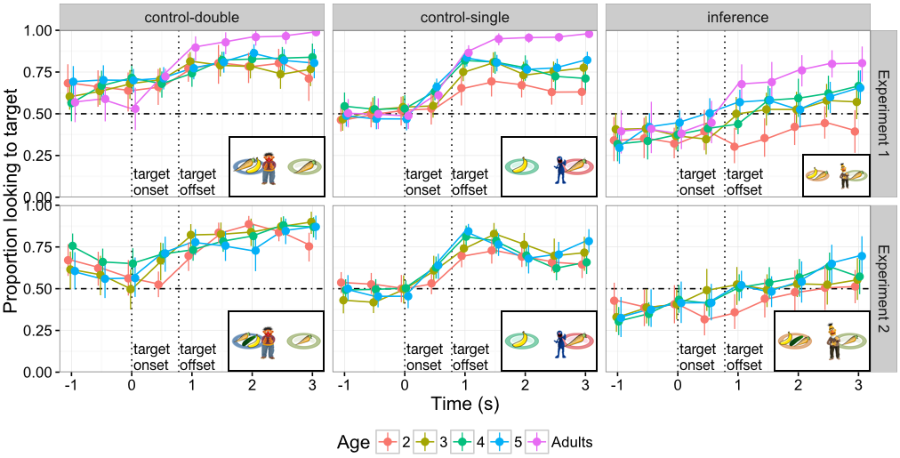
\includegraphics{figs/et_acc-1} 

}

\caption[Proportion of 2- to 5-year-old children and adults looking to the target image as the utterance unfolds in Experiments 1A and 1B (rows), in different trial types (columns)]{Proportion of 2- to 5-year-old children and adults looking to the target image as the utterance unfolds in Experiments 1A and 1B (rows), in different trial types (columns). Time 0 represents the target word onset, and time 0.78 represents the average target word offset. Proportion correct looking is defined by looks to the target divided by the total looks to both the target and the distractor. Example stimuli are shown in the bottom right hand corner for each condition; the named character emerged at the end of the trial to mark the correct target.}\label{fig:et_acc}
\end{figure}
\end{CodeChunk}

\subsubsection{Accuracy}\label{accuracy}

First, we looked at the rate of accurate looking toward the target in
each of trial types. Participants of all ages looked to the targets in
both control-double and control-single trials reliably above chance
(50\%; Figure 1). Children of 4 years and above robustly looked to
targets in inference trials (for 4-year-olds: \(t\)(27) = 2.66, \(p\)
=0.013). For example, upon hearing ``Bert's plate has a carrot,''
4-year-olds looked to the plate with only a carrot more than the plate
with a carrot and a banana.

There were two additional interesting trends in children's looking
patterns: First, 2-year-olds did not disengage from distractors relative
to their baseline bias prior to hearing the target word (also see
Appendix), and were marginally \emph{below} chance in their overall
performance (\(t\)(22) = -3.59, \(p\) = 0.002). Second, even though
older children's correct look to inferential target exceeded look to
distractor, it was lower than expected from previous studies; in Stiller
et al. (2015)'s paradigm, for instance, 4-year-olds selected the correct
referent at approximately 75\%, whereas in the current paradigm, even
5-year-olds looked to the target barely above 60\%.

\begin{table}[tb]
\centering
\begin{tabular}{lrrr}
 Predictor & Estimate & Std. Error & $t$ value \\ 
  \hline
Intercept & 0.62 & 0.05 & 13.64 \\ 
  Control-double & 0.13 & 0.06 & 2.26 \\ 
  Inference & -0.29 & 0.07 & -4.45 \\ 
  Age & 0.04 & 0.01 & 3.08 \\ 
  Control-double * Age & -0.02 & 0.01 & -1.66 \\ 
  Inference * Age & 0.02 & 0.02 & 1.14 \\ 
   \hline
\end{tabular}
\caption{Predictor estimates with standard errors and significance information for a linear mixed-effects model predicting accurate looking to target in Experiment 1A.} 
\label{tab:exp1_tab}
\end{table}

We fit a linear mixed-effects model\footnote{All mixed-effects models
  were run using the \texttt{lme4} package, version 1.1-10 (D. Bates,
  Maechler, Bolker, Walker, \& others, 2014). The random effects
  structure for this model was as follows:
  \texttt{(trial type \textbar{} subid) + (age \textbar{} item)} All of
  our data and processing and analysis code can be viewed in the version
  control repository for this paper at:
  \url{https://github.com/ejyoon/simpimp}.} to measure the effects of
trial type and age on the proportion of children looking to the target
between 0.8 and 4 seconds after the target noun onset (Table 2). We
selected this time window because participants would have to wait until
the end of target noun (0.8 seconds on average) to know they should
switch to the inferential target, given the absence of a disambiguating
continuation (e.g., ``Elmo's plate has a carrot and banana.''). The
mixed model found a significant main effect of trial type and main
effect of age: participants looked to the target significantly less in
inference trials compared to control-single trials, and across all trial
types, participants' looking to target increased with age.

One potential concern was that after each trial, feedback was given to
indicate which of the two potential referents was the target, and thus
it was possible that participants learned to identify the target based
on the feedback. A linear mixed-effects model predicting accuracy based
on order (first vs.~second half of the trials) and age indicated no
significant main effect of order, and no interaction between age and
order (largest \(\beta\) = 0.061, \(p >.20\)).

\subsubsection{Switch time}\label{switch-time}

Next, we wanted to look at the participants' processing speed: how
quickly they made their responses upon hearing the utterance. For this,
we selected trials on which participants were looking at the distractor
at the point of disambiguation, and measured the average length of time
prior to a switch to the target (Fernald, Zangl, Portillo, \& Marchman,
2008).

A linear mixed-effects model measuring the effects of trial type and age
on switch time\footnote{with the same random effects as the model for
  predicting accuracy} as revealed significant main effects of trial
type (\(\beta\) = 0.62, \(p =.004\)) and age (\(\beta\) = -0.08,
\(p =.004\)) on the average RT, with no interaction (largest \(\beta\) =
-0.07, \(p >.24\)). Inference trials were overall slower than control
trials, and participants reacted faster with increasing age in all trial
types.

\begin{CodeChunk}
\begin{figure}[H]

{\centering 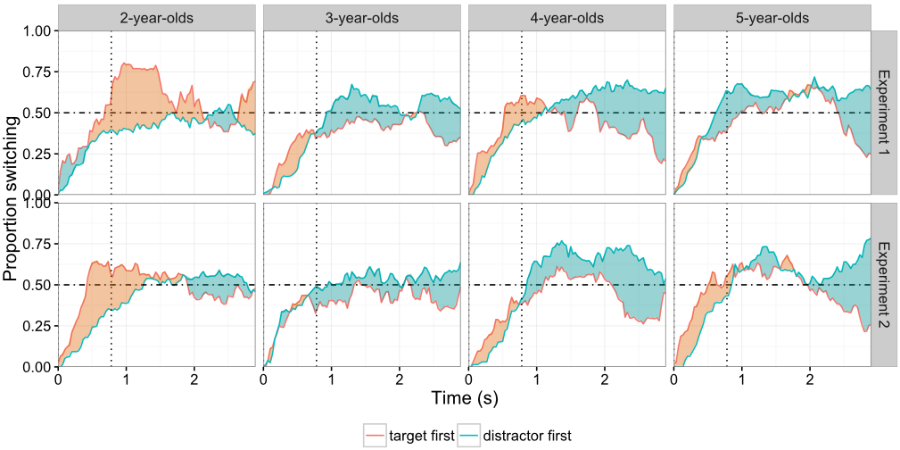
\includegraphics{figs/et_ons-1} 

}

\caption[Onset contingency plot showing results from Experiments 1A and 1B]{Onset contingency plot showing results from Experiments 1A and 1B. Trials were divided depending on where the participant was first looking: the green line indicates trials in which participants looked at distractor first and made switch to target, and orange line target first and switched to distractor. the size of the green shaded region indicates more switches made from distractor-to-target than target-to-distractor. The size of the orange shaded region represents more switches made from target-to-distractor than distractor-to-target.}\label{fig:et_ons}
\end{figure}
\end{CodeChunk}

One question is whether 2-year-olds had difficulty switching correctly
from the distractor to target, or whether they switched incorrectly away
from the target to distractor. To explore this question, we looked at
target- and distractor-initial trials separately, contingent on which
item the child was looking toward from the onset of the target noun
(Fernald, Thorpe, \& Marchman, 2010). The top panels in Figure 2 show
the mean proportion of participants that switched from where they
started in Experiment 1A. Thus, the increase in shift on
distractor-initial trials is a correct response, whereas increase in
shift on target-initial trials is an incorrect response.

Across all age groups, there was an initial increase in shift for both
target-initial and distractor-initial trials, until the offset of the
target word. Then age groups diverged in their looking pattern, and
two-year-olds' struggle was evident: whereas older children's switches
to distractor decreased and switches to target increased, two-year-olds'
switches to distractor continued to \emph{increase} after the target
offset, whereas shift from distractor to target stayed the same.

\subsection{Discussion}\label{discussion}

In Experiment 1A, we replicated previous finding that children of 4
years and older compute ad-hoc implicatures. We additionally confirmed
that children of 2 to 5 years successfully compute unambiguous familiar
meanings online (Fernald, Pinto, Swingley, Weinbergy, \& McRoberts,
1998). However, we found that across all ages, rates of correct looking
in inference trials were lower than accuracy rates reported in previous
studies. This may be due to a methodological limitation of eye-tracking,
namely that participants can constantly switch their attention back and
forth between potential referents, especially within the context of
ambiguous meaning, instead of making a single decision to be for a
one-time response to be recorded. We return to this issue in Experiment
2.

Consistent with the implicature processing literature, children below 3
years struggled to make ad-hoc implicatures in the current task.
Interestingly, rather than looking equally at the inferential target and
distractor, 2-year-olds looked more to the distractor, and unlike other
age groups, made more switches from the target to distractor even after
hearing the target noun. Thus, 2-year-olds seem to have had difficulty
disengaging from the distractor that was relatively more salient. These
findings support the inhibitory hypothesis, namely that young children
struggle with implicature tasks because they need to inhibit responses
to a relatively more salient object. In Experiment 1B, we sought to test
this hypothesis using the salience manipulation discussed in
Introduction.

\section{Experiment 1B}\label{experiment-1b}

In Experiment 1A, we confirmed previous findings that children of 4
years and above succeed in ad-hoc implicature computation whereas
younger children struggle. We also saw preliminary evidence that younger
children's failures can be attributed to their difficulty to inhibit
attention away from the distractor. Experiment 1B further explored this
inhibitory hypothesis. We used the same stimuli as Experiment 1A but
added an extra feature to the distractor in inference trials to make it
more salient, in order to increase the salience contrast between the
target and distractor. For example, when the inferential target was a
plate with only a carrot, the distractor was a plate with a carrot,
banana, \emph{and cucumber}.

As explained earlier, the salience manipulation will lead to different
predictions based on which aspect of the context is primarily used:
salience vs.~pragmatics. If children are influenced more by
\emph{salience} due to the difficulty of inhibitory control, then they
will incorrectly look more toward the salient distractor. On the other
hand, if children are influenced more by contextual strengthening of
implicature, upon hearing ``Grover's plate has a carrot'' and
recognizing two unnamed extra features (banana and cucumber) on the
distractor, then they will correctly identify and attend to the
inferential target (plate with only a carrot) as the referent.

\subsection{Method}\label{method-1}

\subsubsection{Participants}\label{participants-1}

Participants were recruited as in Experiment 1A. A total of 129 children
were recruited but a few of them were excluded from the sample for the
following reasons: age other than 2 to 5 years (\emph{n} = 2),
parent-reported English exposure less than our prespecified criterion of
75\% (\emph{n} = 17), noncompliance or difficulty with the experimental
procedure (\emph{n} = 1), experimenter error or technical issues
(\emph{n} = 1). The final sample consisted of 100 (out of 108 qualifying
participants; see Table 1).

\subsubsection{Stimuli}\label{stimuli}

The stimuli were identical to Experiment 1A, except for one change:
distractor items in inference trials and target items in control-double
trials now had three features instead of two (see bottom panels in
Figure 1).

\subsubsection{Design and Procedure}\label{design-and-procedure}

The design and procedure were identical to Experiment 1A.

\subsection{Results and Discussion}\label{results-and-discussion}

\subsubsection{Accuracy}\label{accuracy-1}

As in Experiment 1A, children of all age groups identified the target in
both types of control trials (Figure 1). There was limited evidence that
older children made implicatures in the inference trials, but not
younger children (4-year-olds: \(t\): \(t\)(28) = 2.01, \(p\) =0.054;
2-year-olds: \(t\): \(t\)(24) = -0.87, \(p\) =0.392).

A linear mixed-effects model predicting accuracy based on age and trial
type in Experiment 1B showed a significant main effect of trial type
(\(\beta\) = -0.28, \(p <.001\)), such that looking at target was lower
in inference trials than in control trials. There was no significant
main effect of age or interaction between age and trial type (largest
\(\beta\) = -0.28, \(p >.19\)). Thus, there was no improvement in
looking to the correct target with age increase. As in Experiment 1A,
there was no order effect (largest \(\beta\) = 0.09, \(p >.05\)).

\subsubsection{Switch time}\label{switch-time-1}

A linear mixed-effects model predicting the switch time, or time to make
the first switch from the distractor to target after the target noun
onset, based on age and trial type found a significant main effect of
trial type (\(\beta\) = 0.57, \(p =.028\)) and age (\(\beta\) = -0.1,
\(p =.0078\)) on the average RT, with no interaction (\(\beta\) = -0.08,
\(p >.23\)). Thus, as in Experiment 1A, participants' looking was faster
with increasing age, and looking to inferential targets was slower than
to unambiguous targets.

\begin{table}[tb]
\centering
\begin{tabular}{lrrr}
 Predictor & Estimate & Std. Error & $t$ value \\ 
  \hline
Intercept & 0.62 & 0.05 & 13.22 \\ 
  Experiment 1B & 0.07 & 0.07 & 1.03 \\ 
  Control-double & 0.13 & 0.06 & 2.15 \\ 
  Inference & -0.29 & 0.07 & -4.23 \\ 
  Age & 0.04 & 0.01 & 3.07 \\ 
  Experiment 1B * Control-double & 0.01 & 0.08 & 0.13 \\ 
  Experiment 1B * Inference & 0.01 & 0.10 & 0.09 \\ 
  Experiment 1B * Age & -0.02 & 0.02 & -1.30 \\ 
  Control-double * Age & -0.02 & 0.02 & -1.61 \\ 
  Inference * Age & 0.02 & 0.02 & 1.09 \\ 
  Experiment 1B * Control-double * Age & 0.00 & 0.02 & 0.19 \\ 
  Experiment 1B * Inference * Age & 0.00 & 0.03 & 0.06 \\ 
   \hline
\end{tabular}
\caption{Predictor estimates with standard errors and significance information for a linear mixed-effects model predicting accurate looking to target in Experiments 1A and 1B.} 
\label{tab:exp2_tab}
\end{table}

\subsubsection{Comparison between Experiment 1A and
1B}\label{comparison-between-experiment-1a-and-1b}

To determine the effect of salience contrast on children's inferential
processing, we compared looking at targets across both Experiment 1A and
1B for inference trials. A linear mixed-effects model predicting
accuracy based on experiment, age, and trial type (Table 3) revealed
significant main effects of trial type and age, but no interaction
between Experiment 1B and any other variable. Thus, in contrast to our
initial predictions, we did not find evidence of the effect of
perceptual salience on children's looking patterns. Additionally, in
both Experiments 1A and 1B, we found lower proportion of look toward
inferential target than expected from older children, rarely exceeding
65\%.

\subsection{Discussion}\label{discussion-1}

In Experiment 1B, across all ages, children looked more toward neither
the inferential target nor the distractor. This was surprising, given
that 4- to 5-year-olds successfully identified the inferential targets
in Experiment 1A. As we predicted earlier, children may rely on either
salience-based or pragmatics-based processing strategy; it is possible
that children were affected by both aspects, but the strengthened
implicature canceled out the effect of salience contrast.

Another possibility is that children relied more on one cue over the
other, but they simply needed more time to explore and process all that
is displayed, especially with more items to be examined. One limitation
of the current paradigm was that the end of each trial was not
contingent upon children's inferential decision, and did not guarantee
sufficient time for its completion. To keep the task engaging and
fast-paced, every trial in Experiment 1A and 1B had an approximately
three-second window for recording children's eye gazes, but younger
children may have needed longer to process and interpret the utterance.
To address this potential limitation, we designed another experiment,
where we used another time-sensitive paradigm: a tablet study, which
offers ample time for decision-making while keeping the task engaging.

\section{Experiment 2}\label{experiment-2}

In Experiment 2, we tested the effects of salience contrast using a
tablet paradigm. One advantage of the tablet paradigm over eye-tracking
in Experiment 1A and 1B is the high level of feedback contingency on
participant responses; we provided feedback immediately following
participant responses (transition to the next phase), which not only
made the task more engaging, but also allowed trials to finish after
participants have provided their answers, rather than ending after some
arbitrary amount of time. Participants were also tested on both 2-vs-1
and 3-vs-1 trials, making it possible to test the effect of salient
contrast manipulation within subjects.

\subsection{Method}\label{method-2}

\subsubsection{Participants}\label{participants-2}

Participants were recruited as in Experiment 1A, except that a part of
the sample was recruited from a local nursery school. A total of 123
children were recruited but a few were excluded from the sample for the
following reasons: age other than 2 to 5 years (\emph{n} = 3),
parent-reported English exposure less than our prespecified criterion of
75\% (\emph{n} = 5), parental interference (\emph{n} = 2), noncompliance
or difficulty with the experimental procedure (\emph{n} = 9). The final
sample consisted of 98 (out of 104 qualifying participants; see Table
1).

\subsubsection{Stimuli}\label{stimuli-1}

Items in the visual stimuli used the same set of images as in Experiment
1A, presented on a tablet. Same auditory stimuli were used as in
Experiment 1A.

\subsubsection{Design}\label{design}

The design was identical to Experiment 1B, except that each participant
saw two possible variations of the number of features for each trial
type (2-vs-1 and 3-vs-1 for inference and control-double trials, 1-vs-1
and 2-vs-2 for control-single trials). There were no filler trials.

\subsubsection{Procedure}\label{procedure-1}

An experimenter introduced children to the task using a tablet. Then
they completed two practice trials, where they were asked to select an
obvious, unambiguous referent (e.g., ``cow'' as opposed to ``rabbit''),
followed by 16 test trials.

\subsection{Results}\label{results-1}

\begin{CodeChunk}
\begin{figure}[H]

{\centering 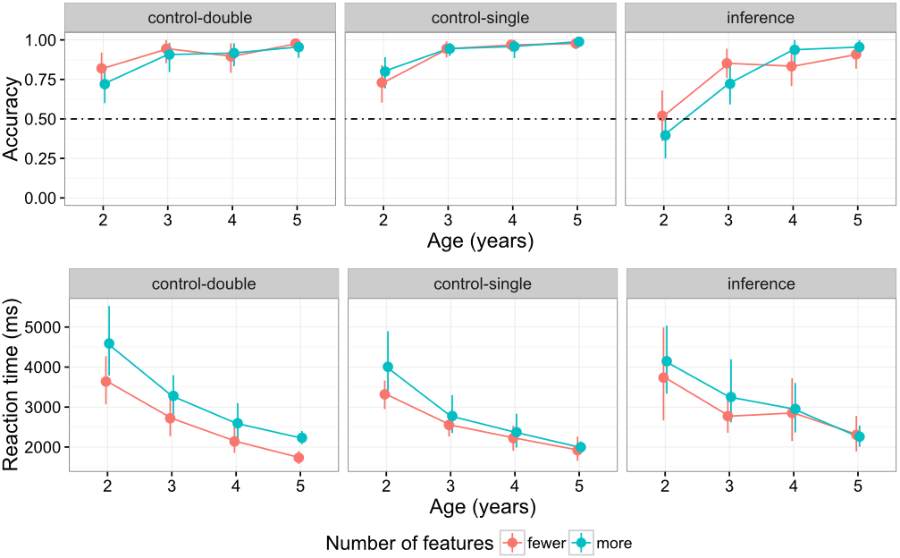
\includegraphics{figs/ipaccrt-1} 

}

\caption[Accuracy rates and reaction times in Experiment 2]{Accuracy rates and reaction times in Experiment 2. Orange lines represent trials in which there were less features present (2-vs-1 for control-double and inference, 1-vs-1 for control-single) and green lines represent trials with more features (3-vs-1 for control-double and inference, 2-vs-2 for control-single).}\label{fig:ipaccrt}
\end{figure}
\end{CodeChunk}

\begin{table}[tb]
\centering
\begin{tabular}{lrrr}
 Predictor & Estimate & Std. Error & $t$ value \\ 
  \hline
Intercept & 0.64 & 0.07 & 8.84 \\ 
  Control-double & 0.11 & 0.09 & 1.25 \\ 
  Inference & -0.26 & 0.11 & -2.34 \\ 
  Age & 0.08 & 0.02 & 3.93 \\ 
  3-vs-1 & 0.07 & 0.09 & 0.78 \\ 
  Control-double * Age & -0.03 & 0.03 & -1.23 \\ 
  Inference * Age & 0.04 & 0.03 & 1.22 \\ 
  Control-double * 3-vs-1 & -0.20 & 0.13 & -1.53 \\ 
  Inference * 3-vs-1 & -0.27 & 0.13 & -2.10 \\ 
  Age * 3-vs-1 & -0.02 & 0.03 & -0.61 \\ 
  Control-double * Age * 3-vs-1 & 0.04 & 0.04 & 1.12 \\ 
  Inference * Age * 3-vs-1 & 0.06 & 0.04 & 1.78 \\ 
   \hline
\end{tabular}
\caption{Predictor estimates with standard errors and significance information for a linear mixed-effects model predicting accurate selection of target in Experiment 2.} 
\label{tab:exp3_tab}
\end{table}

\subsubsection{Accuracy}\label{accuracy-2}

As in Experiment 1A and 1B, children across all ages were able to
identify the target in control trials. In inference trials, all age
groups showed higher accuracy than in eye-tracking (Figure 3). 4- and
5-year-olds' performances were nearly at ceiling, and even 3-year-olds
chose the inferential target above chance (\(t\)(59) = 6.78, \(p\)
\textless{} 0.001). 2-year-olds' performance did not differ from chance
(\(t\)(51) = -0.37, \(p\) \textgreater{} .39).

A linear mixed-effects model predicting accuracy based on age, trial
type and number of features (salience contrast; 2-vs-1 vs.~3-vs-1)
showed a significant negative interaction of inference trial and 3-vs-1
(\(\beta\) = -0.27, \(p = .036\)). Thus, unlike control trials in which
children's performances did not differ by salience contrast, inference
trials showed lower accuracy overall than 2-vs-1. This result was in
support of our initial hypothesis that salience contrast may lead to
greater struggle with the implicature task due to a higher demand for
inhibiting response to distractor with greater salience.

\subsubsection{Reaction time}\label{reaction-time}

Developmental gains in speed of implicature processing were clear: with
increasing age, children computed implicatures and identified the target
faster (Figure 3). As we suspected earlier, 2- and 3-year-olds needed
longer time than 3 seconds on average to indicate their answers, which
may partially explain younger children's flat performances in
Experiments 1A and 1B. A linear mixed-effects model predicting reaction
time based on age, trial type and number of features present showed a
significant main effect of age (\(\beta\) = -476.7, \(p < .001\)). Thus,
children identified the correct referent faster increasingly with age
across all trial types.

\subsection{Discussion}\label{discussion-2}

Developmental gains in speed and accuracy in utterance processing for
both control and inferential trials were clear in Experiment 2. Accuracy
increased and reaction times decreased with age, indicating that
children become more skilled at implicature computation as they get
older. All age groups showed higher accuracy rates in Experiment 2
compared to Experiments 1A and 1B. One possible reason is that
``accuracy'' in a referent selection paradigm that requires a conscious
decision-making (tablet) is different from ``accuracy'' in an
eye-tracking paradigm that tracks an unconscious decision-making
process.

We also found the effect of salience contrast that we predicted earlier:
namely that greater salience contrast leads to greater difficulty for
children to inhibit reacting to the more salient distractor and choose
the less salient target. This means that children were affected more by
salience in salience-pragmatics tradeoff, and their struggle with
inhibitory control outweighed the implicature strengthening support. Why
did older children, who are very much capable of computing implicatures,
not benefit from this implicature strengthening more? Perhaps their
performance, which was already at ceiling, could not be improved
further.

Why did the effect of salience contrast show up in tablet paradigm, but
not in eye-tracking? One possible explanation is that the amount of time
provided for inferential decision-making was too short in eye-tracking.
To provide their answers on tablet, 2- and 3-year-old children often
needed longer than 3 seconds, which was the average amount of time
allowed on eye-tracking for children to indicate their ``answers'' with
their eye gaze. Another possibility is that the salience-pragmatic
interaction may affect decision processes differently in an eye-tracking
vs.~tablet paradigm. This possibility may be related to the reason why
4- and 5-year-old children consistently gave accurate answers on tablet
across both 2-vs-1 and 3-vs-1, whereas they showed evidence of
implicature computation only in 2-vs-1 but not in 3-vs-1 in
eye-tracking. Perhaps older children's search processes for the referent
(as indicated by eye-tracking), but not their final decisions (as
indicated by tablet), were affected by salience contrasts.

\section{General Discussion}\label{general-discussion}

In two Experiments, we confirmed 3- to 5-year-old children's successes
on ad-hoc implicature computation, and saw substantial developmental
gains in their accuracy and speed. Across both eye-tracking and tablet
paradigms, 4- and 5-year-old children successfully computed ad-hoc
implicatures and identified the inferential targets, consistent with
previous findings. In the tablet paradigm, we found evidence of
successful implicature computation even in three-year-olds. Between 2
and 5 years, there was clear improvement in processing skills with
increasing age, such that correct referent identification was more
accurate and faster in both paradigms. Thus, these findings add to the
existing literature to attest to children's growing proficiency in
pragmatic processing, not only in accuracy but also in speed.

We found evidence for the inhibitory hypothesis, that one cause of
toddlers' struggle with implicature processing is inhibitory control. In
the eye-tracking paradigm, 2-year-olds looked more to the distractor
than the inferential target, and they tended to switch their looking
more from the target to the distractor than from the distractor to the
target. These findings suggested that 2-year-olds struggled to overcome
the effect of distractor salience to look to the inferential target.
Through manipulation of salience contrast between inferential targets
and distractors, we also found evidence in the tablet paradigm that
children have more difficulty with identifying the inferential target
when the salience contrast is greater.

Our findings take an important step toward a comprehensive account of
the development of implicature processing. By 2 years of age, children
begin to be aware that informativeness is important to communication,
but our findings suggest that their poor inhibitory control restrains
processing of complicated pragmatic inferences. By 3-4 years, their
inhibitory control is more developed, and they start to compute ad-hoc
implicatures, albeit slowly, when access to relevant alternatives to the
speaker's words are provided in context (Barner et al., 2011). Children
then continue to develop in many ways that contribute to pragmatic
processing, including via changes in processing speed (Kail, 1991),
executive function (Davidson et al., 2006; Diamond \& Taylor, 1996), and
knowledge of inferential alternatives (Barner et al., 2011; Horowitz et
al., under review; Skordos \& Papafragou, 2016).

Our work also contributes to the literature by broadening of the scope
of methodologies to use to examine children's inferential processes. The
eye-tracking and tablet paradigms showed improvements in implicature
processing across age, not only in accuracy but also in speed. The two
paradigms nicely complemented each other in that some patterns in
children's performances that were masked in one paradigm were revealed
in the other (e.g., 3-year-olds' implicature computation on tablet but
not eye-tracking; see Appendix). These findings indicate the importance
of using a variety of time-sensitive methods to probe children's
pragmatic processing.

There are several limitations to be addressed about our work. First, our
salience manipulation involved manipulation of the number of features
present on an item, which might have caused a potential confound between
salience and processing time. Children's greater looking to the
distractor might have been caused by a real desire to acquire more
information, rather than the mere perceptual salience of the
distractors. Second, a statistical comparison between the eye-tracking
and tablet findings is not appropriate, because target identification is
measured differently. Eye-tracking measures the proportion of looking
toward target vs.~distractor over a period of time, whereas tablet
measures a single response for referent selection. Thus, it is difficult
to make strong inferences about the discrepancies (e.g., different
accuracy rates). Future work measures in one methodology both the time
course of attentional trajectories and the speed and accuracy of final
referent identification will be useful.

In sum, our work shows evidence that from at least 3 years, children are
able to compute ad-hoc implicatures, and that younger children's
failures are likely related to effects of perceptual salience of
distractor items. Tasks that have typically been used to look at
children's implicature processing have a variety of extraneous
processing demands, which may explain why it has been difficult to see
children's underlying pragmatic abilities beyond those extraneous
skills. Our work demonstrates the importance of using a range of methods
to measure children's pragmatic processing.

\newpage

\section{Appendix A: Subtracting baseline bias in
eye-tracking}\label{appendix-a-subtracting-baseline-bias-in-eye-tracking}

\begin{CodeChunk}
\begin{figure}[H]

{\centering 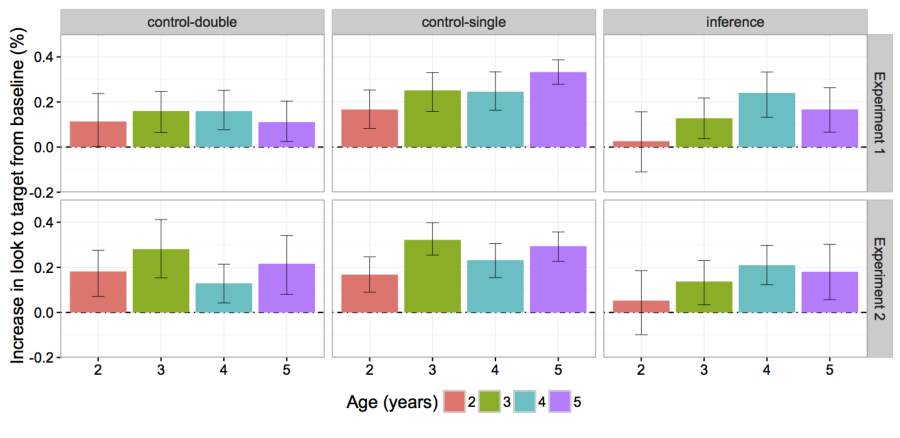
\includegraphics{figs/et_diff-1} 

}

\caption[Increase in look to the target (from the offset of the target noun to 3 seconds after the target noun is produced) compared with baseline looking (from 1 second before the target noun to the start of the target noun)]{Increase in look to the target (from the offset of the target noun to 3 seconds after the target noun is produced) compared with baseline looking (from 1 second before the target noun to the start of the target noun).}\label{fig:et_diff}
\end{figure}
\end{CodeChunk}

In Experiments 1A and 1B, while older children (4- and 5-year-olds)
looked to the inferential target above chance, younger children
(2-year-olds) tended to look to the target below chance and looked more
toward the distractor. The bias in toward distractor was displayed by
all age groups before the start of the target noun in inference trials,
which suggested that all participants were initially drawn toward the
distractor that had more features and thus was more felicitous.

We hypothesized that the difficulty in inhibiting looks to the more
felicitous item caused younger children's struggle to look to the
correct answer. We tested this hypothesis by subtracting initial
baseline looking to target before start of target noun from look to
target after target noun offset. Supporting our hypothesis, increase in
participants' look to target reveals that, whereas 3- to 5-year-olds
increase their look to the target, 2-year-olds do not show change in
attention toward the target (see Figure 4). Thus, it is possible that
2-year-olds' identification of the inferential target was hindered by
the demand to inhibit looks to the salient distractor.

\section{Appendix B: Comparing between eye-tracking
vs.~tablet}\label{appendix-b-comparing-between-eye-tracking-vs.tablet}

\begin{CodeChunk}
\begin{figure}[H]

{\centering 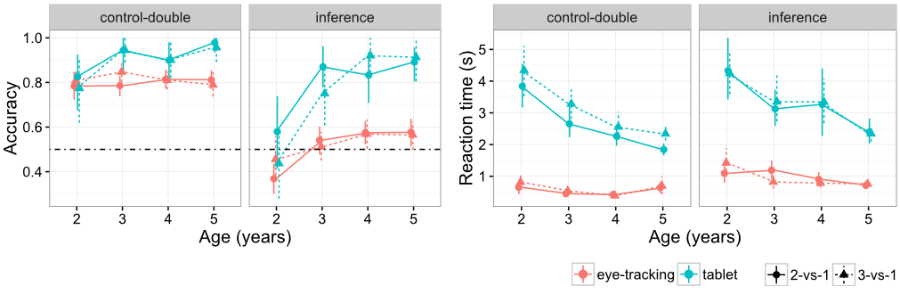
\includegraphics{figs/etip_comp-1} 

}

\caption[Accuracy and reaction times rates for control-double and inference trials (columns) in eye-tracking vs]{Accuracy and reaction times rates for control-double and inference trials (columns) in eye-tracking vs. tablet (iPad) paradigm (colors). Solid lines (circles) represent 2-vs-1 conditions and dashed lines (triangles) represent 3-vs-1 conditions.}\label{fig:etip_comp}
\end{figure}
\end{CodeChunk}

Comparison of accuracy and reaction time measures from the eye-tracking
paradigm (Experiments 1A and 1B) and tablet paradigm (Experiment 2)
shows that robust implicature computation by 3- to 5-year-olds is much
more clearly revealed in the tablet paradigm than in the eye-tracking
paradigm (Figure 5). In fact, accuracy for inferential trials in the
tablet paradigm was overall higher than what was reported in Stiller et
al. (2015), possibly due to stimuli that were even more simplified (two
referent candidates instead of three). The tablet paradigm also revealed
the developmental gains in both accuracy (left in Figure 5) and speed
(right) more prominently than eye-tracking.

\begin{table}[tb]
\centering
\begin{tabular}{lccccc}
 Age bin & Paradigm & M trials (acc) & alpha accuracy & M trials (RT) & alpha RT \\ 
  \hline
2 & eye-tracking & 10.48 & .43 & 3.53 & .45 \\ 
    & tablet & 11.44 & .78 & 15.16 & .29 \\ 
  3 & eye-tracking & 10.44 & .66 & 3.42 & .77 \\ 
    & tablet & 11.55 & .84 & 15.17 & .79 \\ 
  4 & eye-tracking & 10.89 & .61 & 2.87 & -.33 \\ 
    & tablet & 12.00 & .42 & 16.00 & .86 \\ 
  5 & eye-tracking & 10.62 & .57 & 3.55 & -.12 \\ 
    & tablet & 11.84 & .20 & 15.68 & .65 \\ 
   \hline
\end{tabular}
\caption{Standardized reliability coefficients (Cronbach's alpha) for accuracy (acc) and reaction time (RT) by paradigm and age group, along with the mean number of trials for each.} 
\label{tab:etip_rel}
\end{table}

We also examined whether our study measured the variable of interest
with good reliability, by computing Cronbach's \(\alpha\), a statistic
that determines the internal consistency of experimental items (Santos,
1999). Across both eye-tracking and tablet paradigms, our study
contained three trial types (control-single, control-double, and
inference), with 8, 4, and 4 trials respectively, a small number on
which to compute reliability statistics. To assess reliability, we
examined non-inference (control) trials and computed a reliability
coefficient for each experiment and age group, for both accurate looking
and reaction times (see Table 5).

Overall, reliability estimates looked reasonable for accuracy and
reaction time, with a few aspects to be noted. For accuracy, younger
children showed decent reliability in both paradigms, whereas older
children had low reliability in the tablet paradigm, likely due to a
ceiling effect. For reaction time, reliability was generally higher for
tablet paradigms, especially among older children. It should be noted
that reaction time reliability for eye-tracking was computed with very
sparse data (2-3 trials). Thus, the tablet paradigm overall more clearly
and more reliably showed children's success in implicature computation
compared to eye-tracking.

\newpage

\section*{References}\label{references}
\addcontentsline{toc}{section}{References}

Barner, D., Brooks, N., \& Bale, A. (2011). Accessing the unsaid: The
role of scalar alternatives in children's pragmatic inference.
\emph{Cognition}, \emph{118}(1), 84--93.

Barner, D., Chow, K., \& Yang, S.-J. (2009). Finding one's meaning: A
test of the relation between quantifiers and integers in language
development. \emph{Cognitive Psychology}, \emph{58}(2), 195--219.

Bates, D., Maechler, M., Bolker, B., Walker, S., \& others. (2014).
Lme4: Linear mixed-effects models using eigen and s4. \emph{R Package
Version}, \emph{1}(7).

Bott, L., Bailey, T. M., \& Grodner, D. (2012). Distinguishing speed
from accuracy in scalar implicatures. \emph{Journal of Memory and
Language}, \emph{66}(1), 123--142.

Breheny, R., Ferguson, H. J., \& Katsos, N. (2013). Taking the epistemic
step: Toward a model of on-line access to conversational implicatures.
\emph{Cognition}, \emph{126}(3), 423--440.

Chierchia, G., Crain, S., Guasti, M. T., Gualmini, A., \& Meroni, L.
(2001). The acquisition of disjunction: Evidence for a grammatical view
of scalar implicatures. In \emph{Proceedings of BUCLD 25} (Vol. 157, p.
168).

Davidson, M. C., Amso, D., Anderson, L. C., \& Diamond, A. (2006).
Development of cognitive control and executive functions from 4 to 13
years: Evidence from manipulations of memory, inhibition, and task
switching. \emph{Neuropsychologia}, \emph{44}(11), 2037--2078.

Diamond, A., \& Taylor, C. (1996). Development of an aspect of executive
control: Development of the abilities to remember what I said and to
``do as I say, not as I do''. \emph{Developmental Psychobiology},
\emph{29}, 315--334.

Fenson, L., Dale, P. S., Reznick, J. S., Bates, E., Thal, D. J.,
Pethick, S. J., \ldots{} Stiles, J. (1994). Variability in early
communicative development. \emph{Monographs of the Society for Research
in Child Development}, i--185.

Fernald, A., Pinto, J. P., Swingley, D., Weinbergy, A., \& McRoberts, G.
W. (1998). Rapid gains in speed of verbal processing by infants in the
2nd year. \emph{Psychological Science}, \emph{9}(3), 228--231.

Fernald, A., Thorpe, K., \& Marchman, V. A. (2010). Blue car, red car:
Developing efficiency in online interpretation of adjective--noun
phrases. \emph{Cognitive Psychology}, \emph{60}(3), 190--217.

Fernald, A., Zangl, R., Portillo, A. L., \& Marchman, V. A. (2008).
Looking while listening: Using eye movements to monitor spoken language.
\emph{Developmental Psycholinguistics: On-Line Methods in Children's
Language Processing}, 113--132.

Frank, M. C., \& Goodman, N. D. (2012). Predicting pragmatic reasoning
in language games. \emph{Science}, \emph{336}(6084), 998--998.

Frank, M. C., \& Goodman, N. D. (2014). Inferring word meanings by
assuming that speakers are informative. \emph{Cognitive Psychology},
\emph{75}, 80--96.

Frank, M. C., Sugarman, E., Horowitz, A. C., Lewis, M. L., \& Yurovsky,
D. (2016). Using tablets to collect data from young children.
\emph{Journal of Cognition and Development}, \emph{17}, 1--17.

Goodman, N. D., \& Stuhlmuller, A. (2013). Knowledge and implicature:
Modeling language understanding as social cognition. \emph{Topics in
Cognitive Science}, \emph{5}(1), 173--184.

Grice, H. P. (1975). Logic and conversation. \emph{Syntax and
Semantics}, \emph{3}, 41--58.

Hollich, G. J., Hirsh-Pasek, K., Golinkoff, R. M., Brand, R. J., Brown,
E., Chung, H. L., \ldots{} Bloom, L. (2000). Breaking the language
barrier: An emergentist coalition model for the origins of word
learning. \emph{Monographs of the Society for Research in Child
Development}, i--135.

Horowitz, A. C., Schneider, R. M., \& Frank, M. C. (under review). The
trouble with quantifiers: Explaining children?s deficits in scalar
implicature.

Huang, Y. T., \& Snedeker, J. (2009a). Online interpretation of scalar
quantifiers: Insight into the semantics--pragmatics interface.
\emph{Cognitive Psychology}, \emph{58}(3), 376--415.

Huang, Y. T., \& Snedeker, J. (2009b). Semantic meaning and pragmatic
interpretation in 5-year-olds: Evidence from real-time spoken language
comprehension. \emph{Developmental Psychology}, \emph{45}(6), 1723.

Hurewitz, F., Papafragou, A., Gleitman, L., \& Gelman, R. (2006).
Asymmetries in the acquisition of numbers and quantifiers.
\emph{Language Learning and Development}, \emph{2}(2), 77--96.

Kail, R. (1991). Developmental change in speed of processing during
childhood and adolescence. \emph{Psychological Bulletin}, \emph{109}(3),
490.

Katsos, N., \& Bishop, D. V. (2011). Pragmatic tolerance: Implications
for the acquisition of informativeness and implicature.
\emph{Cognition}, \emph{120}(1), 67--81.

Matthews, D., Butcher, J., Lieven, E., \& Tomasello, M. (2012). Two-and
four-year-olds learn to adapt referring expressions to context: Effects
of distracters and feedback on referential communication. \emph{Topics
in Cognitive Science}, \emph{4}(2), 184--210.

Nordmeyer, A. E., \& Frank, M. C. (2014). The role of context in young
children?s comprehension of negation. \emph{Journal of Memory and
Language}, \emph{77}, 25--39.

Noveck, I. A. (2001). When children are more logical than adults:
Experimental investigations of scalar implicature. \emph{Cognition},
\emph{78}(2), 165--188.

O'Neill, D. K., \& Topolovec, J. C. (2001). Two-year-old children's
sensitivity to the referential (in) efficacy of their own pointing
gestures. \emph{Journal of Child Language}, \emph{28}(1), 1--28.

Papafragou, A., \& Musolino, J. (2003). Scalar implicatures: Experiments
at the semantics--pragmatics interface. \emph{Cognition}, \emph{86}(3),
253--282.

Papafragou, A., \& Tantalou, N. (2004). Children's computation of
implicatures. \emph{Language Acquisition}, \emph{12}(1), 71--82.

Pruden, S. M., Hirsh-Pasek, K., Golinkoff, R. M., \& Hennon, E. A.
(2006). The birth of words: Ten-month-olds learn words through
perceptual salience. \emph{Child Development}, \emph{77}(2), 266--280.

Santos, J. (1999). Cronbach\(\backslash\)'s alpha: A tool for assessing
the reliability of scales. \emph{Journal of Extension}, \emph{37}(2),
1--5.

Skordos, D., \& Papafragou, A. (2016). Children?s derivation of scalar
implicatures: Alternatives and relevance. \emph{Cognition}, \emph{153},
6--18.

Sperber, D., \& Wilson, D. (1995). \emph{Relevance: Communication and
cognition}. Oxford: Blackwell.

Stiller, A., Goodman, N. D., \& Frank, M. C. (2015). Ad-hoc implicature
in preschool children. \emph{Language Learning and Development}.

Yurovsky, D., \& Frank, M. C. (2015). Beyond naive cue combination:
Salience and social cues in early word learning. \emph{Developmental
Science}.

\bibliography{simpimp.bib}

\end{document}
